\documentclass{beamer}
\setbeamercovered{transparent}
\usetheme{Berkeley}
\usecolortheme{seahorse}
\usepackage{graphicx} % Required for inserting images
\usepackage{hyperref}

\title{OOPs Project Presentation}
\subtitle{Snakes and Ladders}
\author[Yuvraj, Shreyas, Sneha, Suraj] % (optional, for multiple authors)
{Y.~Chauhan\inst{1} \and S.~Ladhe\inst{1} \and S.~Chinchkar\inst{1} \and S.~Kumar\inst{1}}

\institute[VFU] % (optional)
{
  \inst{1}%
  Computer Science and Engineering\\
  Indian Institute of Information Technology - \\Vadodara, International Campus Diu
}
\date{18th October, 2023}
\logo{
\includegraphics[height=1cm]{logo.png}}
\begin{document}

\maketitle

\begin{frame}
\frametitle{Table of Contents}
\tableofcontents
\end{frame}

\section{Introduction}
\begin{frame}{Introduction}
    \begin{block}{Snakes and Ladders}
   
   \begin{itemize}
       \item The Snakes and Ladders Game is a digital recreation of the classic board game. The primary aim is to provide an enjoyable and interactive gaming experience for players of all ages.

    \item  Snakes and Ladders is one of the most recognizable board games today. Originated in ancient India around
the 13th century AD, the game was designed to teach children the cause and effect of good and bad deeds.   
   \end{itemize}
    \end{block}
\end{frame}

\begin{frame}{Objectives}
    \begin{itemize}
\item Our project aims to demonstrate the effectiveness of an Object-Oriented approach in solving complex problems.
\item  We'll showcase how abstraction and inheritance enhance efficient product design.
\item Object-oriented concepts streamline debugging and optimize the CI/CD Pipeline.
\item  The Web-App interface ensures compatibility across all devices and eliminates support concerns.
\item  A simple Web-App guarantees playability on any device with internet access and a browser.
    \end{itemize}
\end{frame}

\section{Software Requirement Specifications}
\begin{frame}{SRS and Use Case Diagram}
    \begin{itemize}
        \item[1.] Functional Requirements
        \item[2.] Non-Functional Requirements
        \item[3.] Use Case Diagram
    \end{itemize}
\end{frame}
\subsection{Functional Requirements}
\begin{frame}{Functional Requirements}
      \begin{itemize}
        \item \textbf{Die Rolling:} Implement random die roll functionality (1-6).
        \item \textbf{Player Movement:} Move the player's game piece based on the die roll.
        \item \textbf{Consecutive 6s Rule:} Detect three consecutive 6s and void the last 6.
        \item \textbf{Normal Block:} Move the player to the designated block.
        \item \textbf{Snake Head Block:} Move the player to the corresponding snake's tail block.
        \item \textbf{Ladder Bottom Block:} Move the player to the corresponding ladder's top block.
    \end{itemize}
\end{frame}
\subsection{Non-Functional Requirements}
\begin{frame}{Non-Functional Requirements}
        \begin{itemize}
        \item \textbf{User Interface:} Intuitive and visually appealing user interface.
        \item \textbf{Performance:} Smooth game play with responsive controls.
        \item \textbf{Compatibility:} The game should run on popular web browsers.
        \item \textbf{Security:} Ensure data privacy and prevent cheating.
    \end{itemize}
\end{frame}
\subsection{Use-Case Diagram}
\begin{frame}{Use Case Diagram}
    \begin{figure}
        \centering
        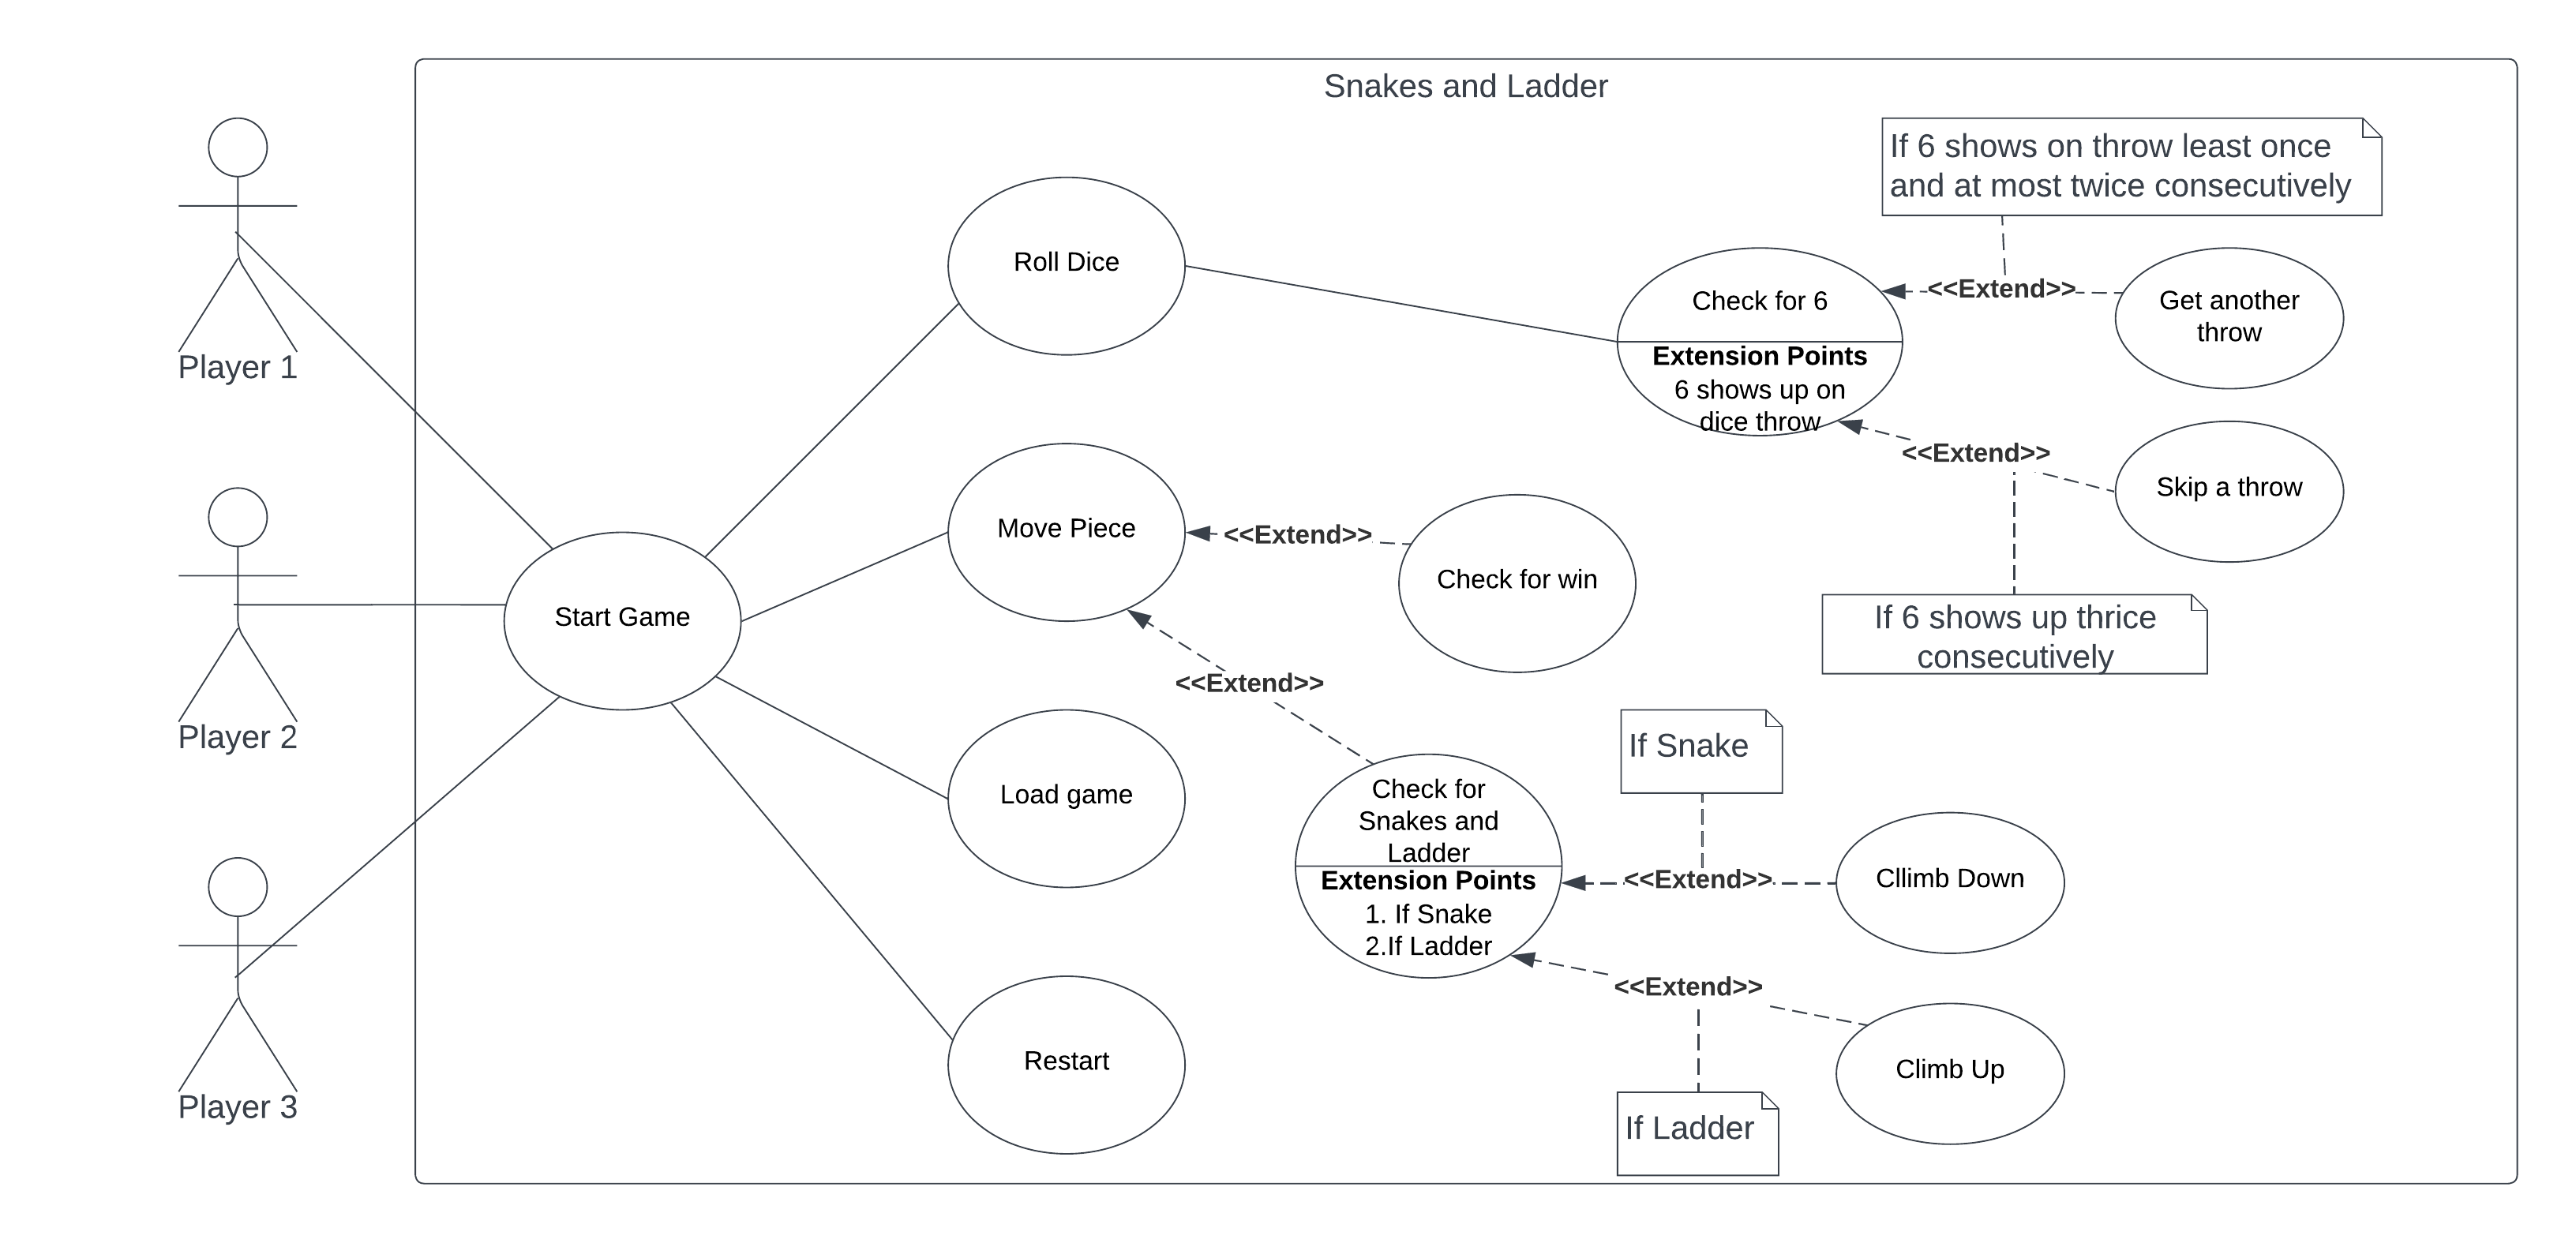
\includegraphics[width = 10cm]{Snakes and ladder.png}
        \caption{Use Case Diagram}
    \end{figure}
\end{frame}
\section{Technology Stack}
\begin{frame}{Technology Stack}
\begin{itemize}
    \item [1.] Front End
    \only<1>{
    \begin{block}{Front End}
    \begin{itemize}
        \item React JS
        \item CSS (Tailwind)
    \end{itemize}
    \end{block}
    }
    \item <2->[2.] Back-End
        \only<2>{
    \begin{block}{Back End}
    \begin{itemize}
        \item Django
    \end{itemize}
    \end{block}
    }
\item<3-> [3.] Version Control
    \only<3>{
\begin{block}{Version Control}
\begin{itemize}
    \item Git
    \item \href{https://github.com/snakes-and-ladders-oops-project/snakes-and-ladders}{GitHub}
\end{itemize}
\end{block}
}

    \item <4-> [4.] UI/UX
     \only<4>{
    \begin{block}{UI/UX}
    \begin{itemize}
        \item Canva
        \item Figma
    \end{itemize}
    \end{block}
    }
\end{itemize}
\end{frame}
\section{OOA}
\begin{frame}{Object Oriented Analysis}
    \begin{itemize}
        \item[1.] Identifying Classes
        \item[2.] Inherited Classes
        \item[3.] Class Diagram
    \end{itemize}
\end{frame}
\subsection{Identifying Classes}
\begin{frame}{Identifying Classes}
    \begin{itemize}
        \item Player
        \item Dice
        \item Cell
        \item Board
        \item Game
    \end{itemize}
\end{frame}
\subsection{Inherited Classes}
\begin{frame}{Inherited Classes}
    \begin{itemize}
        \item Inherited Class from Cell:
        \begin{itemize}
            \item firstCell
            \item Jumper
            \item lastCell
        \end{itemize}
        \item Inherited Class from Jumper
        \begin{itemize}
            \item Snakes
            \item Ladders
        \end{itemize}
    \end{itemize}
\end{frame}
\subsection{Class Diagram}
\begin{frame}{Class Diagram}
    \begin{figure}
        \centering
        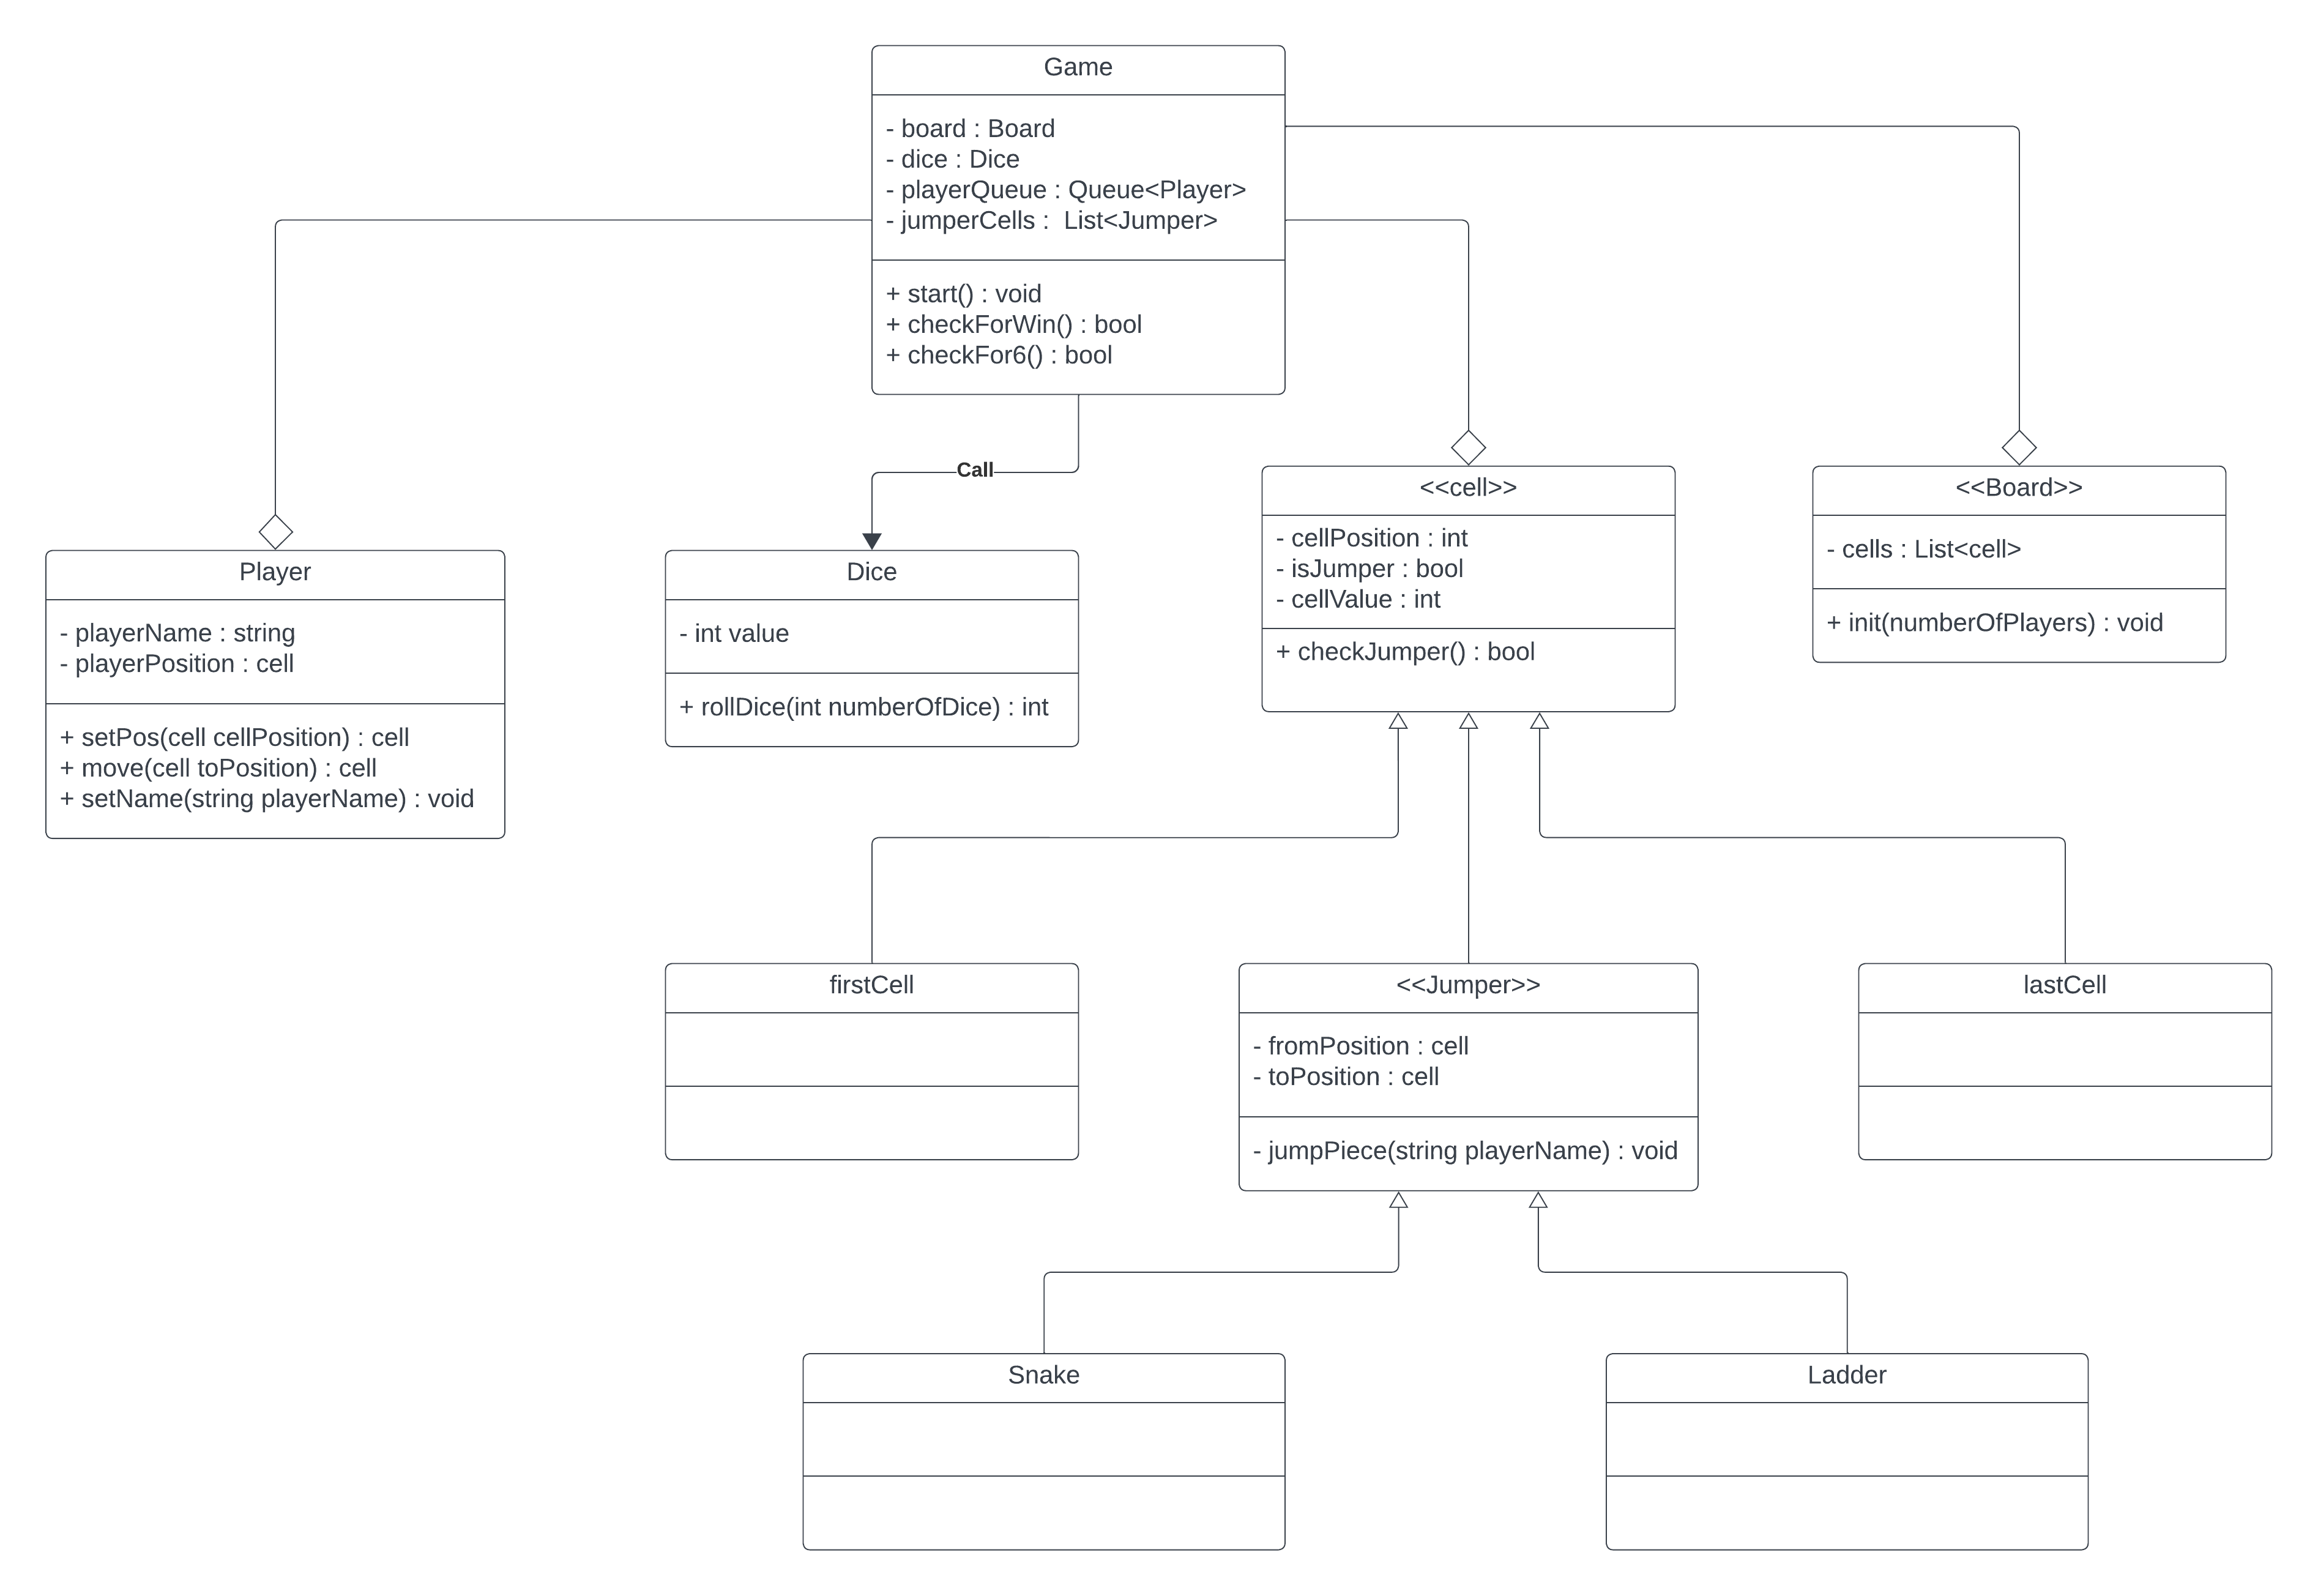
\includegraphics[width = 0.9\linewidth]{UML diagrams.png}
        \caption{Class Diagram}
        \label{fig:enter-label}
    \end{figure}
\end{frame}
\section{Conclusion}
\subsection{Dependencies}
\begin{frame}{Dependencies}
    \begin{itemize}
        \item Requires a modern browser to run.
        \item Multiplayer functionality is not available
        \item Interface might get overloaded due to multiple requests (dice roll).
    \end{itemize}
\end{frame}
\subsection{Future Aspects}
\begin{frame}{Future Aspects}
    \begin{itemize}
        \item Multiplayer functionality
        \item Save game progress and loading saved game
        \item Incorporating Cloud hosting and saving game progress on Cloud.
    \end{itemize}
\end{frame}
\subsection{Conclusion}
\begin{frame}{Conclusion}
\begin{block}{Conclusion}
    
Our Object-Oriented "Snakes and Ladders" project demonstrates the power of OOP principles for efficient, maintainable games. Future plans include multiplayer, saved game progress, and cloud integration.
\end{block}

\end{frame}
\end{document}
